\documentclass[11pt, a4paper]{article}

\usepackage{amsmath}
\usepackage{amsfonts} %Matheschriften
\usepackage{amssymb} %Mathesymbole
%\usepackage{mathptmx} % Einstellung für Schriften und Sonderzeichen in mathematischen Umgebungen
                        % ändert SChriftfont
\usepackage{wasysym} % Stellt diverse Sonderzeichen bereit
\usepackage{siunitx}
\usepackage{float}
\usepackage{microtype}
\usepackage{graphicx}
\usepackage{hyperref}


\usepackage[ngerman]{babel}
\addto\captionsngerman{%
 \renewcommand{\abstractname}{Abstract}}

\title{Versuch 2: Pendel}
\author{Jascha Fricker, Benedict Brouwer}

\begin{document}
    \maketitle

    

    \begin{abstract}
        In diesen beiden Versuchsaufbauten werden verschiedene Pendel untersucht. Zum einen wird mit
        einem Reversionspendel die Erdbeschleunigung $g$ gemessen, zum anderen werden zwei mit einer Feder
        gekoppelte Pendel untersucht und mit den Messwerten u.a. die Federkonstante berechnet. 
    \end{abstract}

    \tableofcontents

    \section{Reversionspendel}

    \subsection{Experimenteller Aufbau und Theorie}

    Ein Reversionspendel hat zwei Aufhängepunkte und zwei Massen, die alle auf einer Geraden liegen.
    Dabei kann ein Masse verschoben werden.
    Es gibt zwei Positionen des verschiebbaren Gewichts, an dem die Periode der Schwingung an beiden
    Aufhängepunkten gleich ist. Für ein Reversionspendel in dieser Konfiguration ist die Periode
    \begin{align}
         \tau^2 &= 4\pi^2 \cdot \frac{l_r}{g} \\
        \Rightarrow \ \ g &= 4\pi^2 \cdot \frac{l_r}{\tau^2} \label{gformel}
    \end{align}
    (Herleitung siehe \cite[Abschitt 1.3]{pen}). Daraus ist ersichtlich, dass, wenn dieser Fall eintritt, die Periodendauer unabängig von der Masse und des
    Trägheitsmoments ist. So kann mit der Periodendauer und dem Abstand der beiden Aufhängungspunkte $l_r$
    die Erdbeschleunigung ausgerechnet werden.
    Um diese besonderen Positionen der zweite Masse zu finden, wird im Experiment die Periodendauer
    mit der Masse an verschieden Positionen von beiden Aufhängungen gemessen,
    um dann mithilfe des Schnittpunkts der Ausgleichgeraden die gewünschten
    Punkte  zu bestimmen.



    \subsection{Ergebnisse}

    \begin{figure}[ht]
        \centering
        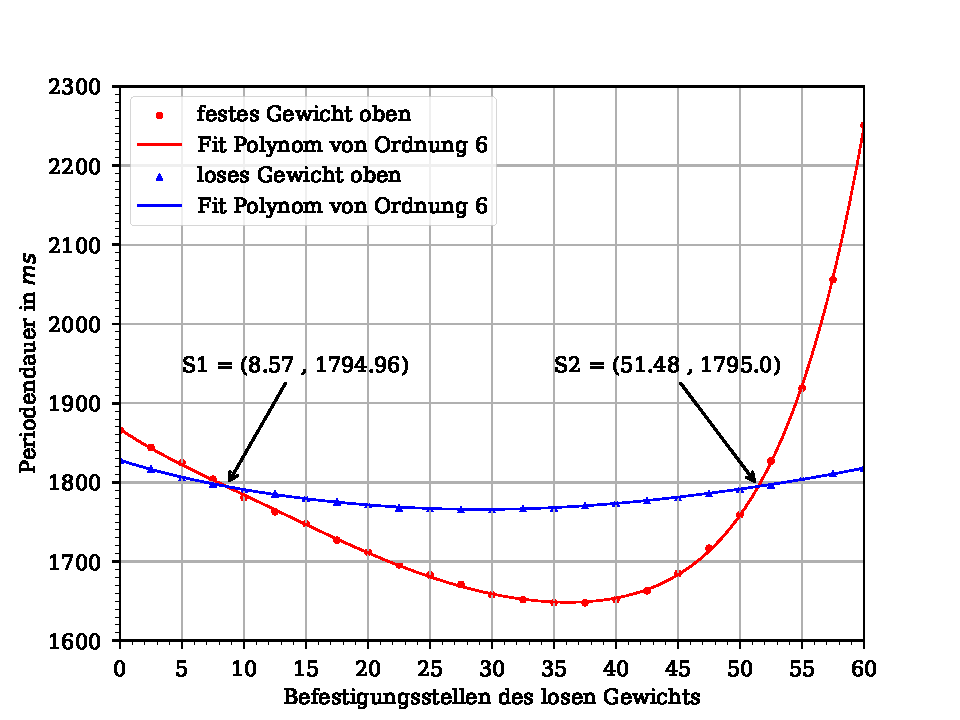
\includegraphics[width=120mm]{./Reversion_grob.pdf}

        \caption{Grobe Darstellung der Messdaten (der Abstand ist nur relativ)}
        \label{fig:revgrob}
    \end{figure}
    \begin{figure}[htb]
        \centering
        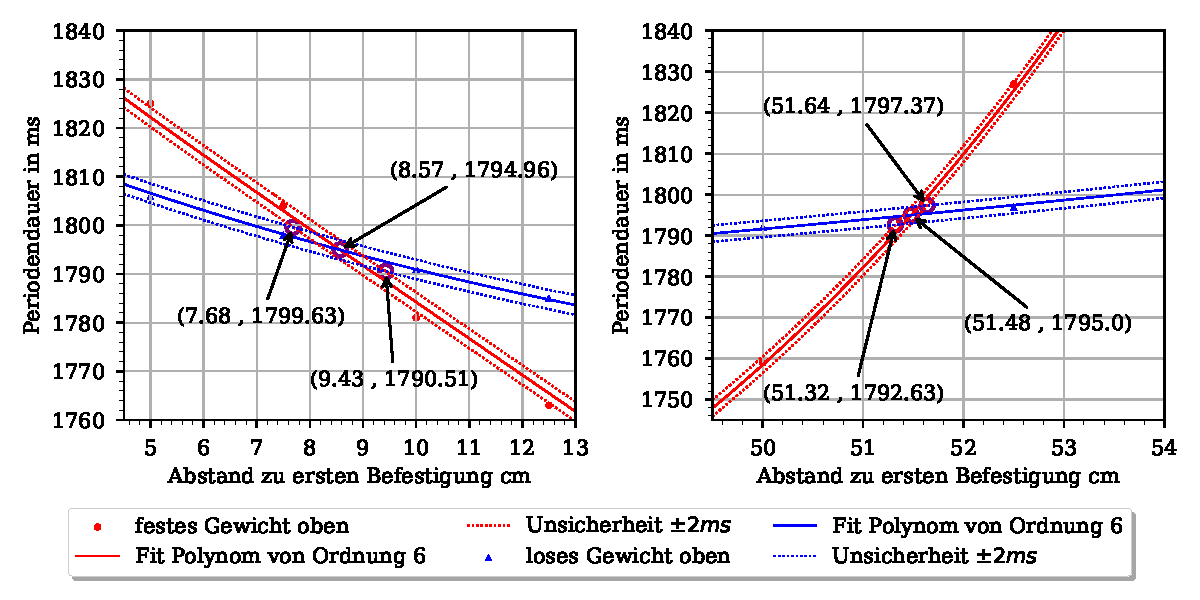
\includegraphics[width=\textwidth]{./Reversion_fein.pdf}

        \caption{Genauere Darstellung der Schnittpunkte}
        \label{fig:revfein1}
    \end{figure}

    Im Graphen \ref{fig:revgrob} wurde die Periodendauer abhängig vom Ort der zweiten Masse für beide Aufhängungspunkte dargestellt. 
    In dem Graphen \ref{fig:revfein1}  können die beiden Schnittpunkte der Periodendauer der verschiedenen
    Aufhängungen nochmal näher gesehen werden. Die Daten wurden mit ienem Polynom 6. Grades gefittet.
    Leider ist dies aber noch nicht genau genug, sodass einige Punkte ausserhalb
    der Konfidenzintervalls liegen. Dies ist uns aber erst nachher aufgefallen. Für den Fehler der Zeitmessung
    wurden $2 \si{\milli\second}$ angenommen, da in den Messdaten eine maximale Abweichung von $1\si{\milli\second}$ bei verschiedenen Messungen 
    der gleichen Periodendauer vorkam und die Lichtchranke selber auch eine Genauigkeit von $1\si{\milli\second}$ hat.
    Beachtenswert ist, dass das Pendel einge Zeit braucht bis es sich eingependelt" hat und konsistente Messwerte
    gemessen werden können. Der Abstand der beiden Aufhängungspunkte $l_r$ beträgt $800,0(11)\si{\centi\metre}$.

    \begin{table}
        \centering
        \begin{tabular}{c c c}
            & Schnittpunkt 1 & Schnittpunkt 2 \\ \hline
            Periodendauer &  $1794,96(456)\si{\milli\second} $ & $1795,00(234)\si{\milli\second} $ \\
            Erdbeschleunigung & $9,803(51)\si{\metre\per\second\squared}$ & $9,802(26)\si{\metre\per\second\squared}$ \\
            gewichtetes Mittel & \multicolumn{2}{c}{$g = 9,802(23)\si{\metre\per\square\second}$}
        \end{tabular}
        \caption{Ergebisse}
        \label{ergrev}
    \end{table}

    
    Der in München vom International Gravimetric Bureau gemesse Wert von $g = 9,807232\si{\metre\per\second\squared}$ \cite{glit} liegt
    eindeutig im Konfidenzintervall unserer Messungen, die in Tabelle \ref{ergrev} dargestellt sind, und sogar relativ nahe am berechneten Wert.


    \section{Gekoppelte Pendel}

    \subsection{Experimenteller Aufbau und Theorie}

    In diesem Experiment wurden zwei Pendel beobachtet, die mit eier Feder auf einer einstellbaren Höhe
    verbunden wurden. Solche Pendel haben zwei Fundamentalschwingungen. 
    Die gleichphasige Winkelgeschwindigkeit 
    \begin{align}
        \omega_{gl} = \sqrt{\frac{mgl}{J}}
    \end{align}
    
    der Schwingung
    wird nur durch das Trägheitsmoments $J$, die Masse $m$ und dem Abstand $l$ des Schwerpunkts zur Aufhängung bestimmt.
    Die gegenphasige Schwingung mit Winkelgeschwindigkeit. 
    \begin{align}
        \omega_{geg} = \sqrt{\frac{mgl+2\kappa r^2}{J}}
    \end{align}
    beeinflusst hingegegen auch die Feder $\kappa$ und der Befestigunsabstand $r$ letzterer.
    In diesem Versuch müssen drei Messreihen aufgenommen werden: Eine gleichphasige, eine gegenphasige und
    eine mit Schwebung. \\
    In \textbf{Aufgabe 11} soll der Koplungsgrad $K$ bestimmt werden. Diesen bestimmt man mithilfe der beide
    Winkelgeschwindigkeiten

    \begin{align} \label{Kformel}
        K = \frac{\omega_{geg}^2 - \omega_{geg}^2}{\omega_{geg}^2 + \omega_{geg}^2} \ \ \ \text{Siehe: \cite[Formel (35)]{pen}}
    \end{align}
    der gleichphasigen und gegenphasigen Schwingung. \\

    In \textbf{Aufgabe 12} sollen aus der Schwebung mithilfe der Schwebungskreisfrequenz $\omega_S$
    und der mitteleren Kreisfrequenz  $\omega_M$ zuerst die Grundschwingungsfrequenzen
    \begin{align}
        \omega_{geg} &= \frac{\omega_{geg} + \omega_{gl}}{2} + \frac{\omega_{geg} - \omega_{gl}}{2} = \omega_M + \omega_S \\
        \omega_{gl} &= \frac{\omega_{geg} + \omega_{gl}}{2} - \frac{\omega_{geg} - \omega_{gl}}{2} = \omega_M - \omega_S
    \end{align}
    ausgerechnet werden (Siehe: \cite[Formel (34)]{pen}). Um dann wieder den Kopplungsgrad nach Formel (\ref{Kformel})
    zu bestimmen. \\
    Mit den gegeben (Theorie-) Daten in \textbf{Aufgabe 13} \cite{pen} (Masse Pendelgewicht $M_P = 1,080(20)\si{\kilogram}$,
    Masse Stange $M_S = 0,160(5)\si{\kilogram}$, Abstand Gewicht-Aufhängung $l = 0,968(10)\si{\metre}$ und Länge $l_0 0 1,030(20)\si{\metre}$
    lassen sich Trägheitsmoment
    \begin{align}
        J = 1,202(52)\si{\kilogram\metre\squared} \label{J}
    \end{align}
    und Drehmomentkonstante
    \begin{align}
        D = 11,06(30)\si{\newton\metre} \label{D}
    \end{align} 
    ausrechnen (Fehlerberechnung siehe \cite[Formel (19)]{ABW}) und damit $\omega_{geg}$ und $K$
    mithlife der Formeln \cite[(30)]{pen} und \cite[(35)]{pen}
    berechnen:
    
    \begin{align}
        K &= \frac{\kappa r^2}{D + \kappa r^2} \\
        \omega_{geg} &= \sqrt{\frac{D+2\kappa r^2}{J}}
    \end{align}


    \subsection{Ergebnisse}

    Die verschieden Kreisfrequenzen wurden bestimmt, indem die jeweilligen Theoriekurven mit geeigneten
    Bounds an die Daten gefittet wurden, sodass sowohl die Frequenz als auch die Unsicherheit ausgegeben
    werden konnte.
    \paragraph{Messreihe gleichphasige und gegenphasige Schwingung}
    In Graphen \ref{mess1} wurden die anhand der in Aufgabe 5 bestimmten Messreihen
    berechneten $\omega_{geg}$ und $\omega_{gl}$ mit ihren Fehlern aufgetragen (farbige Fehlerbalken). Der Theoriewert der gleichphasigen
    Schwingung $\omega_{gl}^T = 3,033(52)$, der mithilfe von (\ref{D}) und (\ref{J}) berechnet wurde, 
    unterscheidet sich leider sehr stark von unseren Messwerten. Wir vermuten, dass die angegeben Daten nicht
    die Realbedingungen des Versuchs wiederspiegeln. Dieser Fehler führt auch zu Abweichungen des Theoriewerts
    in der Graphen, sowei bei der Berechnung von $\kappa$.


    
    \begin{table}[H]
        \label{mess1}
        \centering
        \begin{tabular}{c c c c c}
            Feder & Abstand $r$ in \si{\centi\metre} & $\omega_{geg}$ in \si{\radian\per\second} &
            $\omega_{gl}$ in \si{\radian\per\second} & $K$ \\ \hline
            
            \input{KdataTabel.txt}
            %\endgroup%
        \end{tabular}
        \caption{gleichphasige und gegenphasige Kreisfrequenz mit Kopplungsgrad}
    \end{table}

    \paragraph{Messreihe Schwebung}
    Auch mit den anhand von $\omega_M$ und $\omega_S$ der Schwebung (Siehe Tabelle ?)
    berechneten $\omega_{geg}$ und $\omega_{gl}$ kann der Kopplungsgrad $K$ berechnen werden,
    jedoch sind hier, wie im Graphen ? zu sehen ist (schwarze Fehlerbalken), großere Ungenauigheiten

    \section{Anhang}
    \subsection{Fehlerberechung 1}
    
    \paragraph{Unsicherheit $l_r$:}
    $l_r$ wurde mit einem Metalllineal gemessen werden. Deshalb kann mithilfe von \cite[Gleichung (40)]{ABW}
    und \cite[Tabelle 5]{ABW} die Unsicherheit des Lineals (Länge L=1m)
    \begin{align}
        u(L) = 0.5\si{\milli\metre}
    \end{align}
    und mit \cite[Tabelle 1]{ABW} die Ablesegenauigkeit
    \begin{align}
        u_a = \frac{0.5\si{\milli\metre}}{2\sqrt{3}} = 0.15\si{\milli\metre}
    \end{align}
    berechnet werden. Das Metallineal hat jede 0.5mm ein Ablesestrich.
    Die Unsicherheiten werden zur Gesamtunsicherheit
    \begin{align}
        u_l = \sqrt{u(L)^2 + u_a^2 } = 0.52\si{\milli\metre}
    \end{align} 
    zusammengefasst.
    \paragraph{Unsicherheit $\tau$:}
    Die Unsicherheiten wurden mithilfe von der Formel in der Aufgabenstellung \cite[Aufgabe 8]{pen} berechnet.

    \paragraph{Unsicherheiten von $g_1$ und $g_2$:}
    Mit der Formel \ref{gformel} kann die allgemeinen Formel für Fehlerfortpflanzung
     \cite[Formel (20)]{ABW} für diesen Fall angepasst werden:
     \begin{align}
         u(\bar{g}) &= \sqrt{\left(\frac{\partial g}{\partial l_r}\right)^2 u(l_r)^2 +
         \left(\frac{\partial g}{\partial \theta}\right)^2 u(\theta)^2} \nonumber \\
         &= \sqrt{\frac{16\pi^4}{\theta^2} u(l_r)^2 + \frac{64\pi^4l_r^2}{\theta^3} u(\theta)^2}
     \end{align}
    \paragraph{Gewichteter Mittelwert:}
    Der Gewichtete Mittelwert und seine Unsicherheit wurde mithilfe von
    Formeln (29) bis (32) im ABW Skript\cite{ABW} berechnet. da $u_{int}$ mit $0.023\si{\metre\per\square\second}$
    größer als $u_{ext} = 0.00019\si{\metre\per\square\second}$ ist, wird $u_{int}$ als Ungenauigkeit angenommen.


    \bibliographystyle{plain}
    \bibliography{literature}


\end{document}